\documentclass[runningheads]{llncs}
\usepackage[T1]{fontenc}
\usepackage{graphicx}

\begin{document}
\title{Exam Assignments}

\author{Phillip Rothenbeck}
\institute{Training for Programming Contests and Interviews}

\maketitle

\section*{Assignment 1}

\subsection*{What is the time complexity of the following code ... ?}%

\subsubsection*{Code 2} \label{1:1:code2}
\begin{verbatim}
    void print_pairs(const vector<int> &vec) {
        for (size_t i = 0; i < vec.size(); i++) {
            for (size_t j = 0; j < vec.size(); j++) {
                cout << "(" << vec[i] << ", " << vec[j] << ") ";
            }
        }
    }
    
\end{verbatim}
The code prints out all pairs, that are possible in the set of numbers appearing in the input vector. To achive this
the program iterates for each number of the vector through the vector, resulting in the runtime complexity of
$\mathcal{O}(n^2)$

\subsubsection*{Code 6}
\begin{verbatim}
    void reverse(vector<int> &vec) {
        for (size_t i = 0; i < vec.size() / 2; ++i) {
            size_t other = vec.size() - i - 1;
            int temp = vec[i];
            vec[i] = vec[other];
            vec[other] = temp;
        }
    }
\end{verbatim}
The code reverses the order of the elements in the entered vector. In each iteration two elements are exchanged,
which means only half of the vector needs to be traversed. The runtime is $\frac{n}{2} \in \mathcal{O}(n)$

\pagebreak
\subsubsection*{Code 8}
\begin{verbatim}
    uint64_t factorial(uint64_t n) {
        if (n == 0) {
            return 1;
        } else {
            return n * factorial(n - 1);
        }
    }
\end{verbatim}
Since only one recursive call is made per function call the recursion tree is only one line, which terminates when
$n = 0$. This happens after $n$ recursive call and concludes in a time complexity of $\mathcal{O}(n)$


\subsection*{For each of the following time complexities: $\mathcal{O}(1)$, $\mathcal{O}(log n)$, $\mathcal{O}(n)$,
    $\mathcal{O}(n log n)$ and $\mathcal{O}(n^2)$ give an algorithmic example.}

\subsubsection*{$\mathcal{O}(1)$}
\begin{verbatim}
    int add(int a, int b) {
        return a + b; 
    }
\end{verbatim}
The function $add$ adds its inputs $a$ and $b$ together. Since this is done in constant time, the time complexity is
$\mathcal{O}(1)$

\subsubsection*{$\mathcal{O}(log n)$}
Binary search has a time complexity of $\mathcal{O}(log n)$. The input array is already sorted. Using this information
the algorithm compares the searched number with only the median of the array, which splits the array in two halves.
Binary search recursively repeats this for the half, that could contain the searched number until it gets an empty
input. The input array is a preorder traversal of a binary tree, which has a height of $log n$. The algorithm wanders
only on one path between root and leaf, which concludes in the runtime of $\mathcal{O}(log n)$.

\subsubsection*{$\mathcal{O}(n)$}
\begin{verbatim}
    int sum(int n, int *arr) {
        int sum = 0;
        for (int i = 0; i < n; i++) {
            sum += arr[i];
        }
        return sum;
    }
\end{verbatim}
For adding all numbers of an array together, an algorithm has to add each number to the sum. Resulting in $\mathcal{O}(n)$.

\subsubsection*{$\mathcal{O}(n log n)$}
The sorting algorithm Merge-Sort sorts an array of n numbers in $\mathcal{O}(n log n)$ time. When sorting the resulting
recursion tree is binary and has the height of $log n$ with $n$ leafs. It has to go through every path from the root
to each leaf (and combine each leaf to a sorted list afterwards in $log n$). This means it has a runtime of
$(log n + log n) \cdot n = 2 log n \cdot n \in \mathcal{O}(n log n)$

\subsubsection*{$\mathcal{O}(n^2)$}
\begin{verbatim}
    int sum(int n, int **m) {
        int sum = 0;
        for (int i = 0; i < n; i++) {
            for (int j = 0; j < n; j++) {
                sum += m[i][j];
            }
        }
        return sum;
    }
\end{verbatim}
This algorithm sums up all elements of an 2D array with n lines and n columns. For that it has to traverse all $n^2$
elements.

\subsection*{Outline the idea of how to retrospectively compute in $\mathcal{O}(n)$ the maximum profit when buying and then selling
    a stock once.}

The algorithm traverses the array of prices ones it saves the minimal price, that it has come across so far and the
corresponding profit, that could have been made. For each price it calculates the profit from the saved minimal price
and stores it, if it is bigger than the currently stored maximal profit it replaces that number. In addition, if the
current price is smaller than the lowest stored price it will replace the current lowest price. This way the array
needs to be traversed only once to calculate the highest profit.

\subsection*{How would you check if string b is a permutation of string a.}

I would check for both strings how often a letter is appearing in it. If the same letters appear in the same amount
in both strings, they are permutations of each other.

\section*{Assignment 2}

\subsection*{How can we exploit bit operations for operations with sets?}

A set can be converted into a bitset. The bitset is a binary number, in which a certain digit shows if an element exists
in the set(1) or not(0). This can be exploited to do fast comparative operations on two sets like $and$ (intersection
of two sets), $or$ (union of two sets) and $xor$ (symmetric difference of two sets). Since this happens with only one
instruction it is significantly faster than when working with other set implementations.

\subsection*{Explain the difference between arithmetic and logical right shifts for negative signed integers.}
When using the logical right shift, uses 0s to fill the "gap" that is created on the left through shifting the
numbers to right. This is working for unsigned numbers, but if the first bit is used as a sign bit this could
potentially change the sign of the number. To prevent this problem the arithmetic right shift fills the "gap"
with the same value as the sign bit.

\subsection*{Outline an algorithm to count the number of bits that are set to 1 in an integer. (no bitset or built-in functions)}
For this I would use a bit cursor, that always has exactly one bit set to 1 and is of the same length as the input
number. The algorithm iterates over each bit and moves the 1 in the cursor to the looked upon digit. The intersection of
the number and the cursor is formed. If it is greater than 0 a counter is incremented by one.

\begin{verbatim}
    uint_8 count_1_bits(uint_32 n) {
        uint_8 counter = 0;
        for (int i = 0; i < 32; i++) {
            cursor = 1u << i;
            if((cursor & n) > 0)  {
                counter++;
            }
        }
        return counter;
    }
\end{verbatim}

\subsection*{Outline an algorithm to reverse the bits in an unsigned integer (swap bits at position i and n - i).}
We have an index i that increments per iteration by one until it has reached the middle of the binary number. Now
we take to cursors $first\_digit$ with a 1 at the $i$'th digit and $second\_digit$ with a 1 at the $n-i$'th. The
$first\_digit$ cursor is shifted n-i times to the right and the $second\_digit$ cursor is shifted n-i times to the
left. Lastly a union of the cursors and the output number is formed. The swapping is performed through the bit shifting.
If the input number has an odd count of digits i runs to $\frac{bit\_length(n - 1)}{2}$

\subsection*{Imagine you have to reorder integers in an array so that the odd entries appear first. How is this problem related to Quicksort’s partitioning function?}
We introduce an index ($first\_even$) that sits at the position, where the first even number sits and all numbers to
the left are odd. The other index($i$) is running across all numbers of the array. Every time $i$ comes across an odd
number it swaps it with the number at the position of $first\_even$ and increments this index by one. The output array
has all its odd numbers appearing first.

\section*{Assignment 3}

\subsection*{Outline an algorithm to convert a string to an unsigned integer (no negative numbers).}
The algorithm subtracts 48 from each character in the string and multiplies it by the corresponding power
of ten before adding it to the output number.

\begin{verbatim}
    Input: String s and its length n
    digit = 10 ^ (n - 1)
    number = 0
    i = 1
    repeat n times:
        c = i'th character of s
        x = (get ASCII value of c) - 48
        number = number + x * digit
        i = i + 1
        digit = digit / 10
    Output: number
\end{verbatim}

\subsection*{Outline an algorithm to convert an unsigned integer to a string.}
The algorithm starts to allocate a string with a number of characters equal to the number of bits of the integer plus one.
Each digit is extracted, 48 is added, and the resulting ASCII interpretation is stored in the corresponding position
in the string.

\begin{verbatim}
    Input: integer x, stored in b bits
    allocate string s with b + 1 characters and initialize the to ' '
    pow = 10
    rest = 0
    repeat b times with index i from b - 1 to 0:
        digit = (x % pow) - resulting
        s[i] = digit + 48 // results in the ASCII value of the digit
        pow = pow * 10
        rest = rest + digit
    Output: s
\end{verbatim}

\subsection*{Explain the characteristics of the character encodings ASCII, Extended ASCII, UTF-8, UTF-16 and UTF-32.}
ASCII uses 7 bits to encode 128 characters, while Extended ASCII uses 8 bits to encode 256 characters. UTF-8 on the
other hand uses its first bits to declare how many bytes are supposed to be read to get the character. UTF-8 is a
superset of ASCII. UTF-16 can use one or two words of each 16 bits to encode one character, while UTF-32 has a fixed size
of 4 bytes for all characters that it can encode.

\subsection*{What advice can you give to modify strings as quickly as possible?}
To avoid the time-consuming process of copying the entire string, string modifications should be handled in-place.
If copying is unavoidable, minimize the number of times the string is copied. This can be
achieved by marking the positions where modifications are to be made and finalizing them during the copying process.

\subsection*{Why are hardcoded regex expressions often much faster?}
Before using a regular expression it has to be compiled into a state machine, which is time-consuming.
If the state machine for a certain regular expression is already known, it is faster to hardcode the
state machine since this eliminates the step of automatically compiling. Additionally, exploiting
certain characteristics of the regular expression can speed up runtime.

\subsection*{Is run-length encoding a good compression method for strings?}
This depends on the string that is supposed to be encoded. For instance the string cannot contain any digits,
also it should not have a high frequency of changing characters. This could result in the encoded string
being longer than the original. For strings that have a lot of longer sequences of alphabetical letters,
run-length encoding may be a good compression method.

\section*{Assignment 4}

\subsection*{How to delete a (non-tail) node from a singly linked list without knowing its predecessor in $\mathcal{O}(1)$ time?}
To achieve this, copy the values of the successor into the node containing the data to be deleted. Then, set the
pointer of this node to the successor of its successor and delete the successor. This reduces the number of nodes
by one and deletes the data of the node to be deleted.

\subsection*{Explain the runner technique using a linked list example.}
The runner technique involves using multiple pointers to iterate through a linked list at different speeds.
This method can be used to find the pivot element that has 1/4 of all nodes to its right. One pointer
(the runner) moves four times for each move the other pointer makes.

\subsection*{If you were to tune the code for speed, how would you implement a stack?}
I would use a \verb|std::vector| to implement a stack. Since this datastructure provides the method that a
stack needs like \verb|push| (as \verb|push_back|), \verb|pop| (as \verb|pop_back|), \verb|empty| and
\verb|top| (as \verb|back|). These functions are efficiently implemented, making them fast enough.

\subsection*{How can we use a std::list in C++ as a queue?}
To implement a queue using the \verb|std::list|, we first need to specify which side of the list should be the entrance point
and which will be the exit. In this example, we use \verb|front| as the entrance and \verb|back| as the exit. To enqueue,
we use the list function \verb|emplace_front| which constructs a new node at the front of the list with the new data. For
dequeuing, we first save the data and then use \verb|pop_back| to delete the note. Finally, we return the data. The
\verb|size| and \verb|empty| data give the information how big our queue is and if it is empty. Thus, all necessary
mechanisms can be implemented using \verb|std::list|.

\subsection*{How does a binary tree and a binary search tree differ?}
A binary tree is a tree in which each node has at most two children. A binary search tree is a type of binary tree that adds
the condition that for every node x, the left subtree only contains nodes that are lower or equal to x, and the right subtree only contains
nodes being greater than x. Therefore, binary search trees are a strict subset of binary trees.

\subsection*{Describe the different types of binary tree traversals.}
There are three types of tree traversals. First is pre-order, meaning that we first process the current node followed by the left
subtree, and then the right subtree. The second is in-order, which processes the left subtree first, then the current node, and finally
the right subtree. Lastly there is post-order, where we start with the left subtree, continue with the right subtree, and finally process
the current node.

\subsection*{How does a trie and a radix tree differ?}
Both a trie and a radix tree hold information for words in a path from the root. However, a trie assigns exactly one node to each character,
while a radix tree is more compressed as it allows for a node to hold more than one letter. As a result, a radix tree requires fewer nodes than
a trie, to store the same words as it merges a path that has no branches into one node.

\section*{Assignment 5}

\subsection*{Describe briefly the heap data structure.}
The heap is a binary tree that has two conditions. Firstly, a child at depth k can only exist if all children at depth of k - 1 exist.
This means that a new 'row' of children can only start, when the previous one is completely filled. Otherwise, a new child will be added from
left to right in the incomplete row. Secondly, each node must be greater than or equal to its children. The time complexity for insertion is
$\mathcal{O}(log n)$ as the heap characteristics must be maintained. Finding the maximum element takes $\mathcal{O}(1)$ time since the element
is always located at the root. Deleting the maximum takes $\mathcal{O}(log n)$ time, while searching for an item has a complexity of
$\mathcal{O}(n)$.

\subsection*{How would you find the k longest words in a data stream? (You cannot back up to read an earlier value.)}
Utilizing a min-heap can accomplish this task. Each word from the stream is added to the heap. The heap size is checked when a word is added to
ensure it does not exceed k. If the size exceeds k, the shortest word in the heap is deleted. Once the whole stream has been processed, the heap
will only contain the k longest words.

\subsection*{How would you address the problem of merging multiple sorted files that are too large for RAM}
To accomplish this task, a min-heap can be defined with only the smallest number of each file, resulting in a heap of the same size as the
number of files to be merged. For merging, I iteratively would take the minimum from the min-heap, delete it and add it onto the resulting file.
Then, I would push the next smallest number from the file that the minimum originated from. Thus, I would only have to have loaded the smallest number
of each file and for each iteration load from the next number, which has a time complexity of $\mathcal{O}(1)$.

\subsection*{What are sorting networks?}
Sorting networks are data-oblivious sorting algorithms for arrays of a set size. Each network is constructed using out compare-and-exchange
(COEX) modules, which compare two input numbers and exchange them if the condition is met. To be able to sort with these modules they have to be
put into a specific order of comparing different elements of the array. This means that a sorting net can be hardcoded.

\subsection*{Why sorting may speed up set operations?} %not checked
Sorting reduces the amount of work that it takes to find a particular item in a set. Searching is a large part of set operations (when not
represented as a bitset), since the availability of the elements of one set must be checked in another set.

\subsection*{What is a minimal perfect hash?}
A hash function maps a key to an entry in a hash table. Now, a perfect hash function accomplish this without mapping different keys to the same entry.
In contrast, a minimal hash function has no spaces in its hash table, that are not mapped on. Therefore, a minimal hash function ensures that two keys
are not mapped to the same table entry and that the table has no unused spaces.

\section*{Assignment 6}

\subsection*{What is an optimal approach (as fast as possible) to compute the n-Queens problem with backtracking?}
To find all correct solutions, we must go through all possibilities and to check which ones are correct. We do this by successively adding a queen row by row on
the field. Starting with an empty field, we open a 'thread' (also called candidates) for each possible position where the queen can stand in the first row.
For each candidate, a 'thread' is added which positions the queen in all possible positions in the second row. Illegal candidates are pruned until all
rows are filled, leaving only the solution. This method is the fastest possible since we avoid following paths that are already known to be illegal.

\subsection*{Describe some ideas how to solve the 15-puzzle with backtracking (tell me what you think is important).}
To utilize backtracking, a metric is necessary to exclude moves that hinder us. Here, we use the Manhattan distance. For each candidate, we calculate the
Manhatten distance of all entries to its target location, giving us the minimum amount of moves required to reach our goal. We will use the to prune
candidates that exceed the maximum number of moves.

\subsection*{Why is efficient parallelization not trivial in most divide and conquer algorithms?}
The reason for this is that divide and conquer algorithms are integrated most of the time by using recursion. Since each recursion step depends on
further recursion step, data dependencies make it hard to parallelize these applications. Furthermore, recursion function make it hard to do efficient
load balancing which could lead to inefficient parallelization.

\subsection*{What is the difference between divide and conquer and decrease and conquer?}
Divide and conquer algorithms break the problems up into smaller and more manageable sub-problems. The each of them are solved and the results combined
to solve the main problem. Decrease and conquer, on the other hand, reduces the problem into smaller problems of the same kind and solves them by mostly
using the same algorithm. The main problem then can be resolved directly.

\subsection*{What is dynamic programming? When is it useful?}
The main primary principle of dynamic programming is to store the outcomes of sub-problems and retrieve them, when the sub-problem recurs, rather than recalculating the
task. It can be applied to recursion and iterative solutions.

\subsection*{Compare the top-down approach with the bottom-up approach used in dynamic programming.}
As previously mentioned, dynamic programming can be applied to both recursive and iterative solutions. For iterative (bottom-up) solutions, the algorithm first solves
smaller sub-problems first and then moves on to bigger problems until the main problem is reached. This approach makes it easier to write cache-efficient code. For
instance, if a sub-problem depends only on the last n sub-problems, then only those results need to be stored. A top-down (recursive) solution works the other way round and
starting with the main problem each step is broken down into smaller sub-problems. The results of these will be saved to prevent duplicate calculations. Therefore,
all results must be stored simultaneously.

\subsection*{Present briefly a greedy heuristic of your choice.}
Using the movie scheduling problem, as an example, a possible greedy heuristic is to select the next earliest job (movie) that does not overlap, with any accepted job, until
no job remains. This approach fits the definition of a greedy heuristic since the algorithm does not question its own choices and only makes decisions based on the local maximum.

\section*{Assignment 7}

\subsection*{How do you decide how to spend your resources?}
I always prioritize to build recyclers over robots, since their blocking ability makes them more powerful. I have split my bot into three phases. In the first phase, I only build if
I have no recycler on the field. It is built in the spot of my domain with most resources, ensuring that I always get the most out of my single recycler. The rest of the scrap is
spent for units to be able to conquer the most cells. In the second phase, my domain and the enemies are touching, and I build a recycler in any empty cell with a border to the enemy. The bot will build as many recyclers
as it can in a turn. The rest is spent for units again. In the last phase, all scrap is spent into units to be able to conquer as many cells as possible and simultaneously not losing
any cells to recyclers.

\subsection*{How do you decide in which directions your bots move.}
As mentioned before, my bot is split into three phases. In addition to that, I partition my units into three groups: Pawns, that only move to cells, without an owner and that are not the target of another unit. Defenders, that always
peer to my border cells with the highest density of enemy units in the neighboring cells. Attackers, that move into empty enemy cells, but run from enemy units (into the enemy domain). I use the first phase to conquer as many
cells as possible before I meet the enemy. Therefore, all of my units are pawns and one tries to quickly reach the middle of the field. In the second, each robot is classified depending on their position (Robots farther away from the
enemy are pawns; Defenders are next to enemy units; Attackers are next to empty enemy cells). For the third phase, the pawn class only exists as long as reachable unclaimed cells exist, otherwise there are only defenders and attackers,
chosen like in the step before.

\subsection*{Are there situations where your bots behaved in a suboptimal way? Why does this happen? (At any point of the challenge)}
When I came into silver league, my attacker robots were chasing enemy units. Some enemies had their units programmed to run away from my units. This resulted in a never ending chase and my domain being overrun by enemies.

\subsection*{What are some heuristics to improve your bots performance? If you implemented them: how did it work? If you did not implement them, argue why you think they should work.}
I implemented the all heuristics that I thought of. Looking at the behavior of a pawn, a greedy heuristic is applied, since the pawn decides on the momentary state of field which cell to move to next. Also, spawning a unit is a greedy heuristic.
I calculate which of my cells are most likely to be overrun by enemy units (difference the between number of units in my cell and the number of enemy units in neighboring cells) and try to counterbalance this by spawning units in the cells in danger.
If no such cells exist, spawn in connected component with unclaimed cells and no unit inside.

\subsection*{What did you learn from observing other peoples bots? (At any point of the challenge)}
One thing I learned was to cut off my enemy by building a wall of recyclers. I enhanced this by leaving a whole for my units to attack. Also, while building the wall, I try to increase my domain. As mentioned before, I took the idea running away
from my opponent instead of chasing him down, from an opponent.

\section{Assignment 8}

\subsection*{If you need an efficient algorithm to find the shortest path between two nodes in a graph where all edges have length 1, which algorithm would you use and why?}
If the shortest path between two nodes needs to be computed, I would use BFS because it is a simple method and can handle the graph, as edge lengths are uniform.

\subsection*{Assume that you need to find a shortest path in a relatively small graph with arbitrary edge lengths, and you have to have a working algorithm very soon. Which algorithm would you choose and why?}
I would use Dijkstra's algorithm, as it can handle non-uniform edge lengths, and is theoretically is the fastest algorithm to solve this task (only for one pair of nodes), from the pool of algorithms we learned in the lecture. Especially on a
small graph, compared to Floyd-Warshall.

\subsection*{Why does Dijkstra's algorithm not work with negative edge lengths? Give a small example.}
The Dijkstra relies on the greedy heuristic, to always take the next node, with the smallest edge length, that is neighbor to an already connected node. It will always select a node connected with an edge with negative length. Which based on
the interpretation of the graph could disturb the shortest path computation. Example:
\begin{center}
    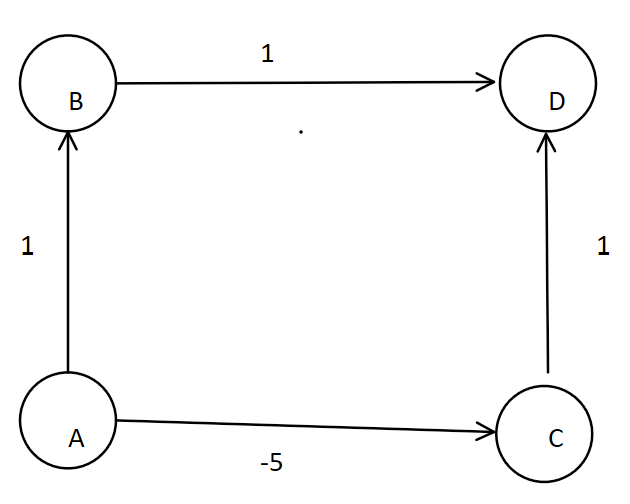
\includegraphics{./resources/graph_0}
\end{center}
Here the path from A to D via C will always be selected as shortest path, since its length equals to -4. Resulting in a negative length for the path.

\subsection*{Present an extension for Dijkstra's algorithm (pseudo-code or description) that also returns a list of nodes that form a shortest path. Explain (proof sketch) why that algorithm is correct.}
\begin{verbatim}
    each node is a pair of its distance to s and its index 

    Input: adjacency matrix of input graph, start node s, sink node t

    define priority queue Q, that sorts its elements by their distance
    define an array D, holding the distances for each node
    define a list P, that will hold all nodes of the shortest path
    set flag t_found to false
    put s into Q with distance 0
    append s to P

    while Q is not empty do:
        get the top node n of Q
        if not already set,
            put the distance of n into D
            if t_found is false: 
                if n has an edge to the last node of P,
                    append n to P
                if n == t, 
                    set t_found to true
            append n to Q
        for each node m do:
            if n has an edge to m,
                if in D not already set,
                    distance d of m = m's distance to n + n's current distance
                    put m into Q with distance d
                    
    Output: D, P
\end{verbatim}

Dijkstra still works since the structure of the algorithm is not changed, only additional data is added. P only
gets the next the nearest node of the graph, which is directly connected to the last added node of P. Also no additional
nodes are added when t has been found. Since the changes do not change the process of the algorithm, it terminates just
like Dijkstra does.

\section*{Assignment 9}

\subsection*{Argue why topological sortings only exist for acyclic graphs.}
A topological sorting algorithm sorts the nodes of a graph in such way, that for each node n all predecessors are positioned in front of it and
all successors of it lay behind it. If the input graph would be cyclic all node of the circle would be both predecessor and successor of each other.
This would lead to an unclear or incorrect ordering.

\subsection*{Briefly describe how you approached and solved Project Euler Problem 1.}
The function solve($n$) computes the sum of all multiples of 3 and 5, that are less than $n$. It iterates through the index $i$ from 1 to $n$, and
adds the corresponding multiples of 3 and 5 to the sum. If the respective multiple is greater than $n$, it is skipped. If both multiples are greater than $n$, the
loop is aborted. For each multiple of 5, the function checks whether it is also a multiple of 3 as well. If this is the case, it is ignored to avoid adding the same number to the sum.

\subsection*{Describe your approach on Project Euler Problem 107: which algorithm did you use and why?}
Since the tasks requires searching for a sub-graph where all nodes are connected and unnecessary edges have been removed, while ensuring minimal edge weights,
a minimal spanning tree must be found. In class, we discussed Prim's algorithm and Kruskal's algorithm. As no runtime limit was specified and Prim's algorithm
was easier to implement, I chose it.

\section*{Assignment 10}

\subsection*{Describe one change that significantly decreased your program length (apart from the obvious: deleting comments or whitespaces). What did you change and how many characters did it save?}
The change was to use one variable for all unnecessary inputs and temporary variables. In general, I tried to reuse variables as often as possible, to reduce the amount of variable definitions that need
to be done, saving me around 30 characters.

\subsection*{Assume you are participating in a code-golf challenge where you have to write an algorithm (in C++) that finds the shortest path between two specified nodes in a graph. Which of the discussed algorithms (see Lecture 8) would you implement, and why?}
I would use the Floyd-Warshall algorithm. It calculates all distances between all nodes, being way more than needed, but it requires the least code to work, as it works with only 3
nested for loops. This can be reduced to a minimal, compared to Dijkstra for example.

\section*{Assignment 11}

\subsection*{Research the difference between the algorithms by Edmonds-Karp and Ford-Fulkerson. Give an example where the Ford-Fulkerson-algorithm might take significantly longer than Edmonds-Karp.}
Edmonds-Karp is a certain implementation of Ford-Fulkerson, using BFS to find the augmented path \cite{ref_EK_FF_relation}. While Ford-Fulkerson runs in $\mathcal{O}(EF)$ time with $E$ being the number of edges and $F$ the maximum capacity of the network, Edmonds-Karp runs in $\mathcal{O}(E*V^2)$.
The worst case for Ford-Fulkerson is given by \cite{ref_FF_worst_case}:

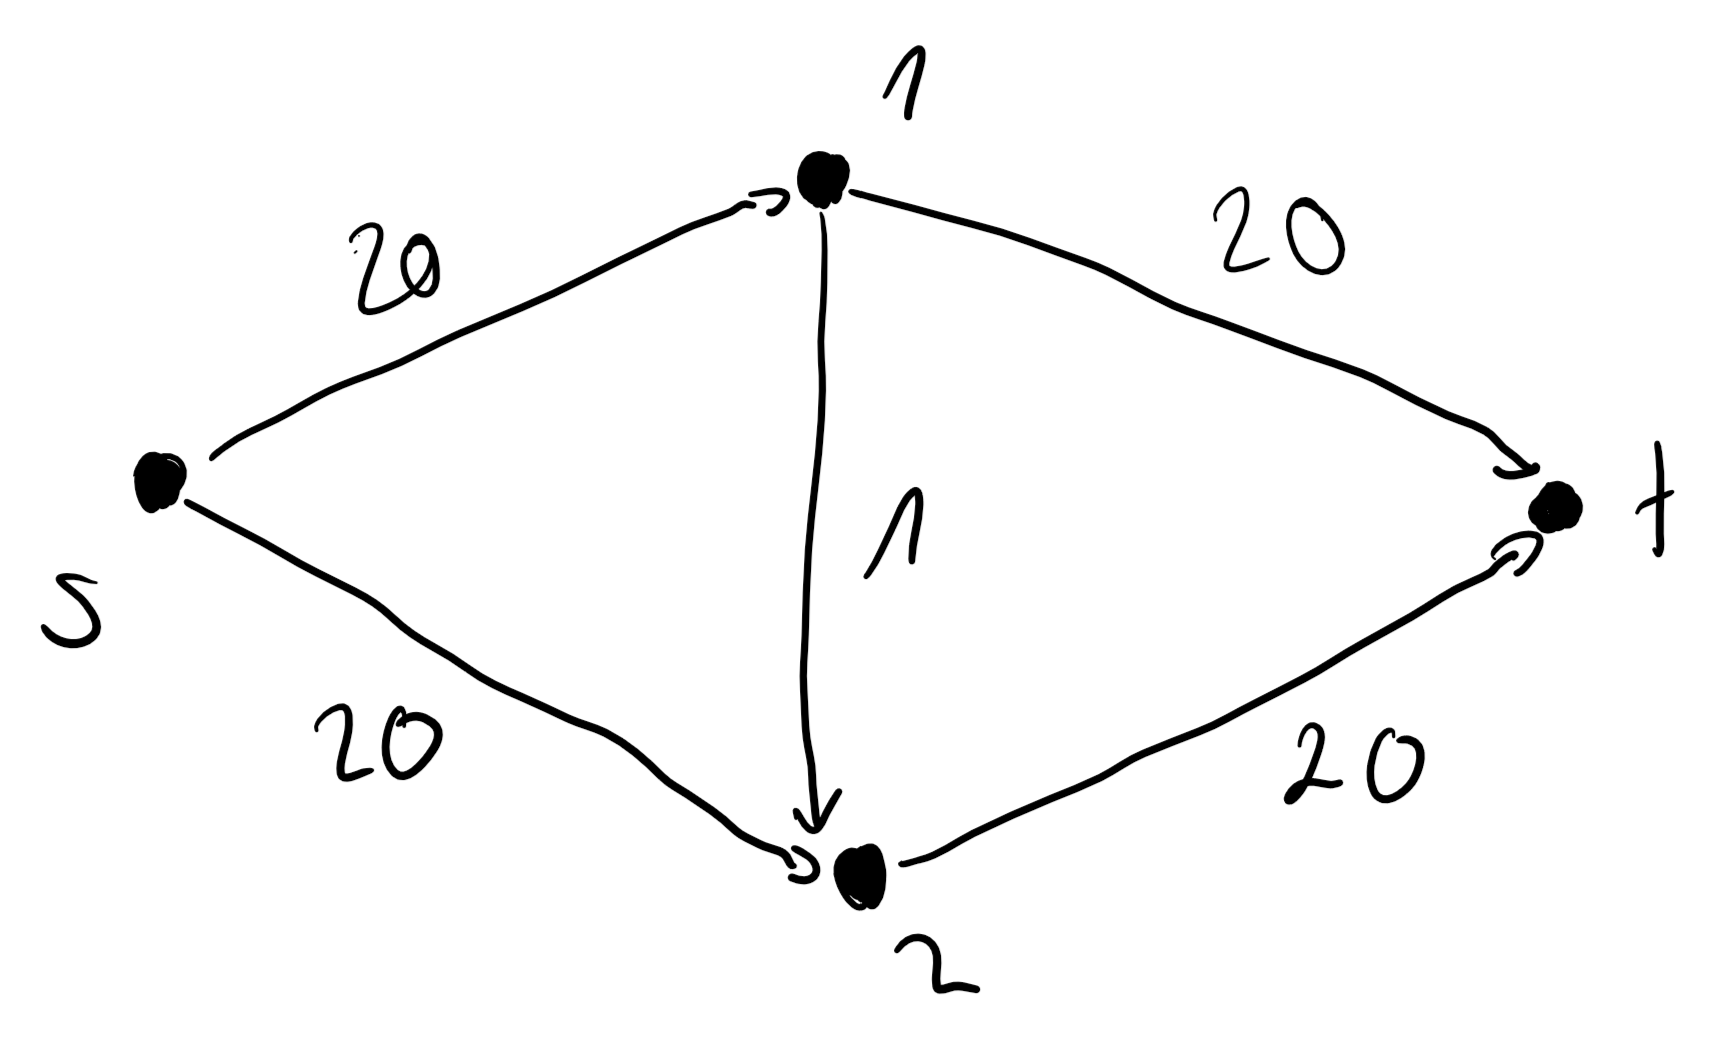
\includegraphics[scale=0.5]{./resources/graph_5}

The first augmented path to be found would s-1-2-t turning the edge between 1 and 2 around. The second would be s-2-1-t, turning the edge again. These iterations would be repeated by the amount of the maximum capacity of the graph, with each step finding augmented paths with maximum flow equal to 1.
Edmonds-Karp on the other hand always chooses the shortest augmented path. This results in a much lower runtime.

\subsection*{Describe your algorithm that solves the Problem 100 ("3n+1-problem"): what algorithmic techniques did you use?}
For each, the algorithm solves the given formula until the $n==1$ is reached. Looking at the results, the algorithm returns the same sequence for the same input. This means that if we come across an already known input, we can add the number of steps it took to complete
the sequence to the steps already taken. For this I defined a hash map that takes a certain n as a key and the number it took to reach 1 as the value. This means I used dynamic programming.

\subsection*{Which algorithm do you use for Problem 459 ("Graph Connectivity"), and why?}
The Floyd-Warshall algorithm was utilized to calculate the distance between two nodes and determine their connectivity. This algorithm was chosen due to its ability to calculate all distances at once, which is advantageous for identifying all connected components within
the input graph. Additionally, a list was implemented to track of all connectivity components that have been identified. In the list each component is represented by one node of the component. To check if a node is connected to a component, its distance to the component's
representative is examined. This process is repeated for every node while simultaneously counting all new components encountered.

\section*{Assignment 12}

\subsection*{Describe the MinCut-Problem and give two examples with a small graph with 5 nodes and 7 edges (the graph has to be connected)}

\subsection*{MinCut}
In a MinCut-Problem a set of edges E of the input graph, that cuts the graph int two components, with the nodes s and t being positioned in different components.
Additionally, E is supposed to have minimal edge weights.

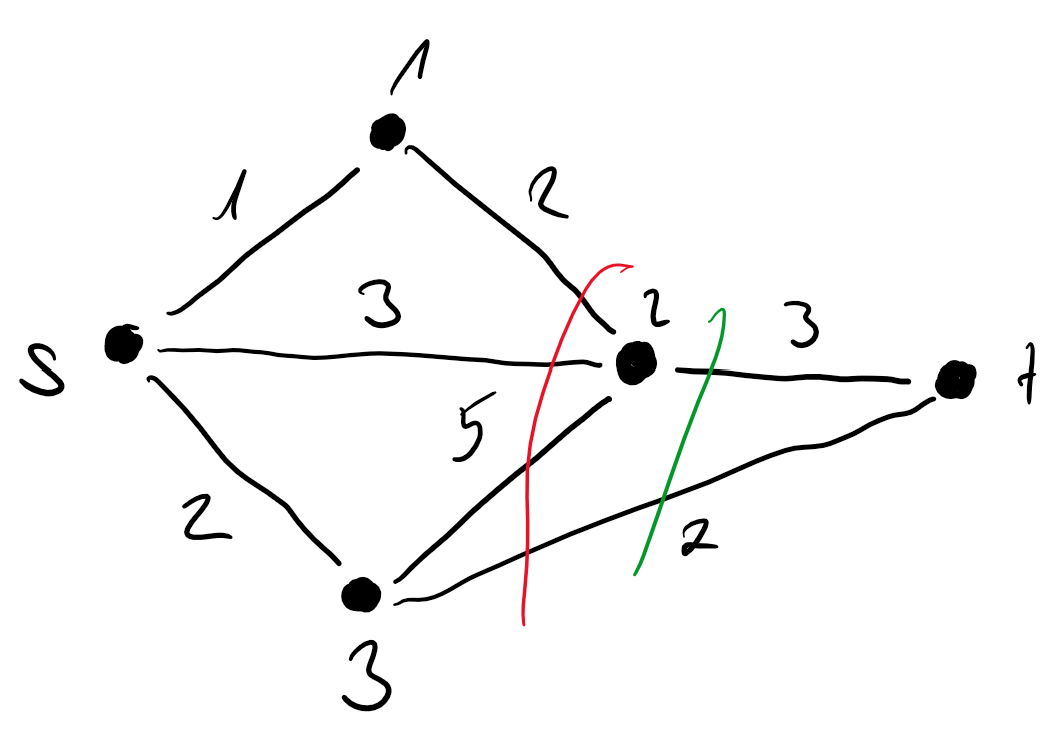
\includegraphics[scale=0.5]{./resources/graph_1}

The green cut is the minimal cut with a weight of 5. The red cut is not minimal with a weight of 12.

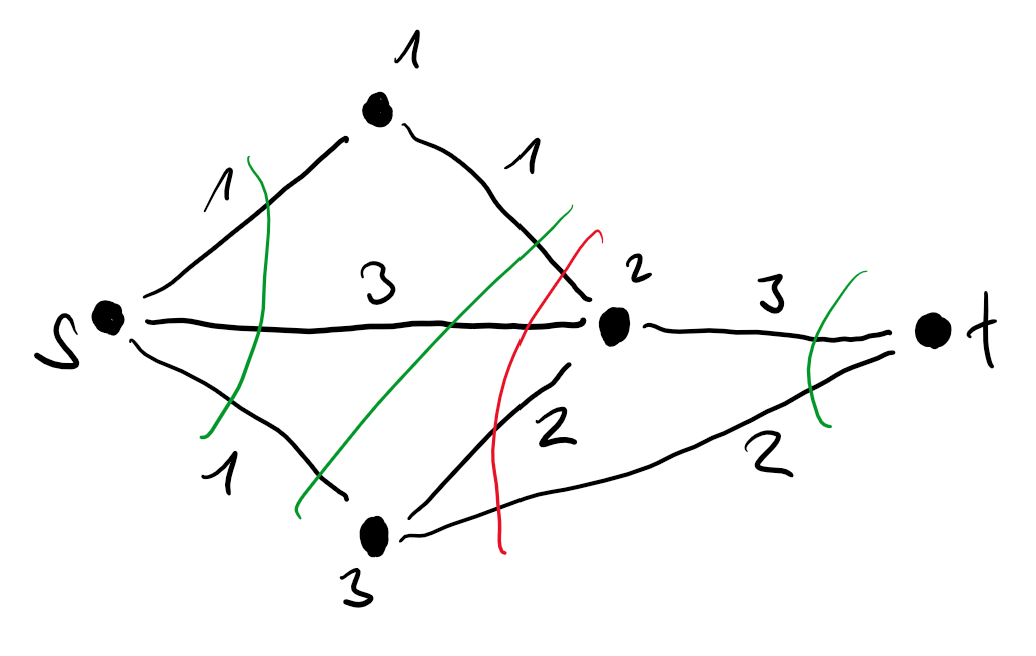
\includegraphics[scale=0.5]{./resources/graph_2}

The green cuts are the minimal cuts with edge weight of 5. The read cut is not minimal with a weight of 8.

\subsection*{Matching}
In a Matching-Problem pairs of nodes are supposed to be found, with the restriction that each edge belongs to at most one matching. A maximal matching is found if there is no other matching with more pairs node. In perfect matchings each node belongs to exactly one pair.

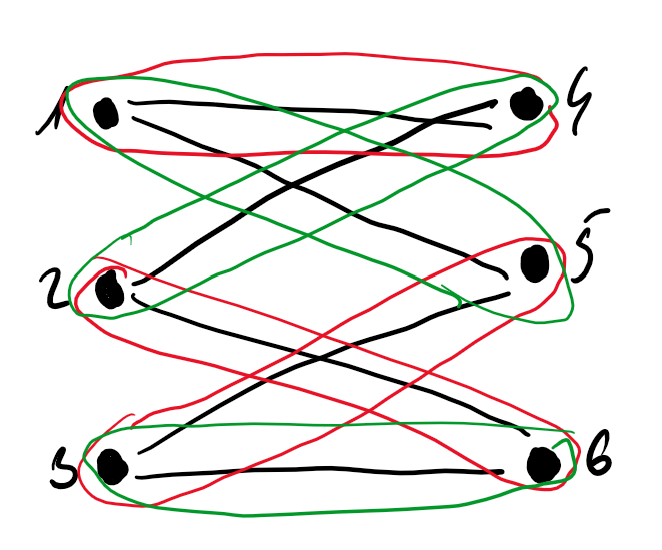
\includegraphics[scale=0.5]{./resources/graph_3}

Each color represents one perfect matching.

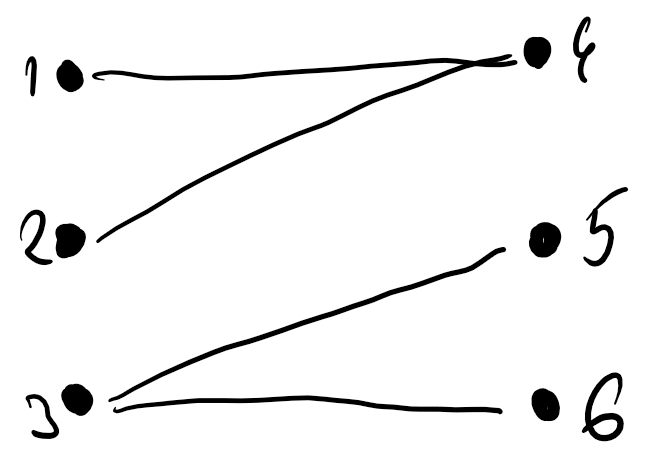
\includegraphics[scale=0.5]{./resources/graph_4}

The following matching exists: (1, 4), (2, 4), (3, 5), (3, 6). Since both 3 and 4 are used twice for a pair, no perfect matching exists, but each node has at least one partner.

\section*{Assignment 13}

\subsection*{Describe a kernel of the $k$-VertexCover-Problem: figure out which nodes have to (and which don’t have to) be in the VertexCover.}

\subsubsection*{Kernel Step 1} Take out all nodes with a degree greater than $k$, these nodes have to be in the VertexCover, as otherwise all of its $k$ (or more) neighbors would then have to be in the cover. Also decrease $k$ by one for each of these.
\subsubsection*{Kernel Step 2} Delete all isolated nodes, as they cover no edges.
\subsubsection*{Kernel Step 3} If after steps 1 and 2 the Graph still contains more than $k^2$ edges, it cannot contain a VertexCover of the size $k$. This is because the graph only contains nodes with a degree of maximal $k$. This can cover $k^2$ edges at most.

\newpage
\subsection*{Design an algorithm (pseudo-code) that constructs a minimal vertex cover for graphs where all nodes have degree at most 2. Your algorithm should run in time $\mathcal{O}(n^c)$ where $n$ is the number of nodes in the graph, and $c$ is a constant (bonus point if you achieve $c = 1$). Prove the correctness and the runtime of your algorithm.}
\begin{verbatim}
    Input: Graph G as an adjacency matrix with set of edges E and set of vertexes V
    define set VertexCover
    add n to VertexCover

    while V is not empty
        if n not defined or if n has no neighbor:
            if there is a node k of degree 1 in V:
                get k's neighbor node n from V
            else:
                get random node n from V
            remove k and n from V
        if n has a neighbor v and:
            if v has a neighbor:
                set the neighbor as the new n
                remove n from V
                add n t VertexCover
            remove v from V
    Output: VertexCover
\end{verbatim}

\subsubsection*{Correctness}
\subsubsection*{Case 1: Linear Graph with uneven number of nodes} The size of the minimal vertex cover is $\lceil\frac{n}{2}\rceil$. This will only be reached if
the two border nodes with degree 1 are not in the vertex cover. This is reached by putting the neighbor of one of these in the cover. From there on every second node
will be put into the cover, ending with the neighbor of the second node with degree 1. This results in $\lceil\frac{n}{2}\rceil$ nodes in the vertex cover.
\subsubsection*{Case 2: Linear Graph with even number of nodes} The size of the minimal vertex cover equals $\frac{n}{2}$. Just like in Case 1, this is reached by taking
every second vertex into the vertex cover.
\subsubsection*{Case 3: Circular Graph} If the Graph is circular the starting node is selected randomly instead of choosing a node next to a vertex with degree 1, as all nodes have the degree 2.

\subsubsection*{Runtime} The base algorithm runs in $\mathcal{O}(|V|)$, as all nodes are only looked at once. But, since we have to find the degrees of some node, which takes $\mathcal{O}(|V|^2)$. The whole algorithm takes $\mathcal{O}(|V|^2)$ setting $c = 2$

\subsection*{Describe your approach at this weeks programming exercise (Problem 1773-A). How does your algorithm find a pair of valid permutations?}

\begin{thebibliography}{8}
    \bibitem{ref_EK_FF_relation} \url{https://cp-algorithms.com/graph/edmonds\_karp.html} 16.02.2024
    \bibitem{ref_FF_worst_case} \url{https://hyperskill.org/learn/step/27203} 16.02.2024

\end{thebibliography}
\end{document}